% Chapter 1

\chapter{Introduction} % Main chapter title

\label{Chapter1} % For referencing the chapter elsewhere, use \ref{Chapter1} 

%----------------------------------------------------------------------------------------

% Define some commands to keep the formatting separated from the content 
\newcommand{\keyword}[1]{\textbf{#1}}
\newcommand{\tabhead}[1]{\textbf{#1}}
\newcommand{\code}[1]{\texttt{#1}}
\newcommand{\file}[1]{\texttt{\bfseries#1}}
\newcommand{\option}[1]{\texttt{\itshape#1}}

%----------------------------------------------------------------------------------------

\begin{multicols}{2}


Lorem ipsum dolor sit amet, consectetur adipiscing elit. Nunc varius commodo lectus ut ultricies. Curabitur pellentesque laoreet auctor. Proin nec ornare sem. Sed pellentesque augue tortor, in faucibus massa auctor quis. Cras scelerisque, leo quis faucibus euismod, lectus mi sodales enim, et cursus quam elit at eros. Phasellus dapibus vitae dui in malesuada. Vestibulum sed ex ac lectus pretium dapibus. Sed aliquet blandit urna ut lobortis. Phasellus orci nunc, varius et nulla nec, blandit fermentum nulla.

\bigskip

\subsection*{How weather radars work}

% full width figure
\begin{figure*}[ht!]
\begin{center}
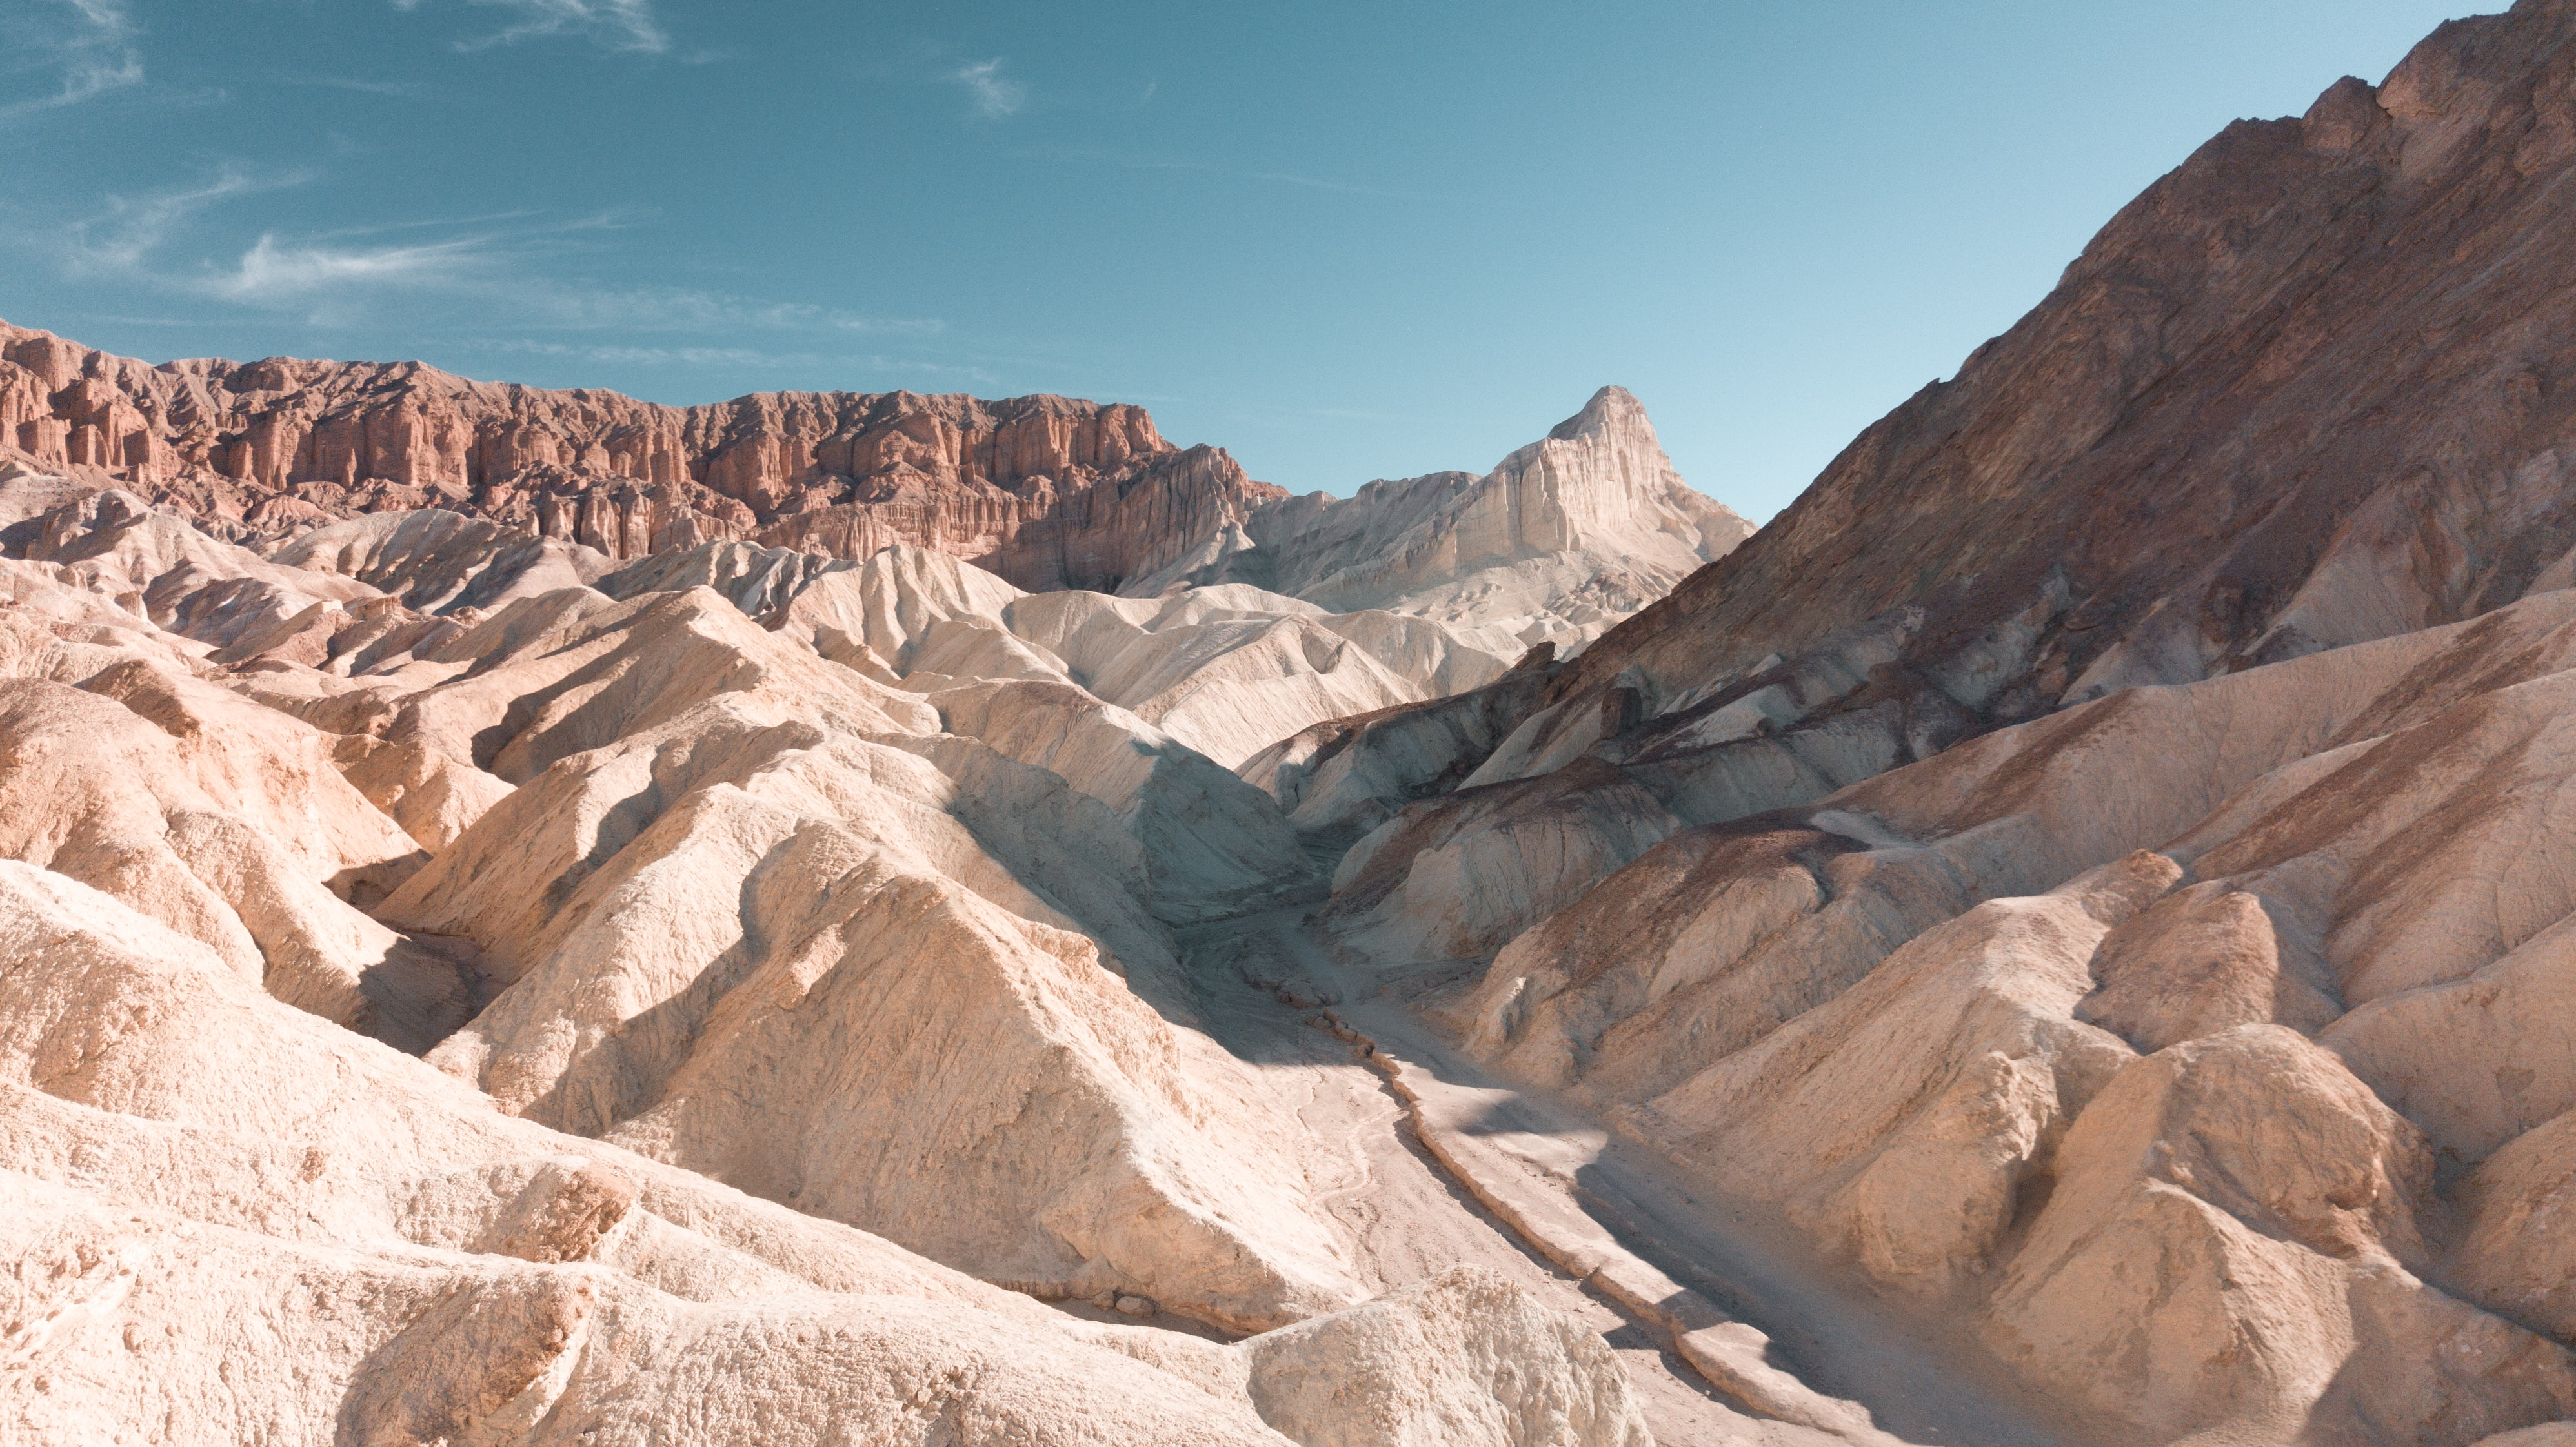
\includegraphics[width=\linewidth]{./Figures/image4.jpg}
\captionof{figure}[Figure with citation.]{This is a figure taken from a different paper, so it needs to be cited. \citep{heistermann_emergence_2014}}
\label{fig:BC_fig1_intro}
\end{center}
\end{figure*}

Vestibulum tincidunt ipsum turpis. Vivamus et nulla sit amet nisl egestas volutpat et eget est. Duis quis sapien vel est fermentum auctor. Quisque volutpat mollis leo in rhoncus. Ut rutrum ligula sed erat molestie, nec tristique dui malesuada. Ut bibendum, eros quis placerat euismod, metus sem rhoncus purus, vel interdum massa risus vitae libero. Integer et imperdiet nibh. Donec venenatis turpis in vehicula dapibus. Nullam luctus porttitor ex, nec cursus nunc semper non. Nam iaculis ligula ut quam feugiat ultricies. Aliquam a blandit massa. Nunc eget ipsum mauris.:

\begin{equation}
    P_r = \frac{z}{r^2} \left ( \frac{P_t g^2 \theta \phi h}{\lambda^2}\right ) \left ( \frac{ \pi^3 } {1024 \ln(2)} \right ) |K|^2 l
\end{equation}

\noindent
where the non-numeric parameters can be classified into three categories:

\medskip

\begin{description}

\item Derived quantities
    \begin{description}
    \item $P_r =$ power received by radar (watts)
    \item $r =$ range or distance to target (m)
    \item $z =$ radar reflectivity factor ($mm^6/m^3$)
    \end{description}
    
\bigskip

\item Radar constants
    \begin{description}
    \item $P_t =$ power transmitted by radar (watts)
    \item $g =$ antenna gain
    \item $\theta =$ horizontal beam width (radians)
    \item $\phi =$ vertical beam width (radians)
    \item $h =$ pulse length (m)
    \item $\lambda =$ wavelength of radar pulse (m)
    \end{description}

\item Assumed values
    \begin{description}
    \item $|K|^2 =$ dielectric constant for radar targets (usually set at 0.93 for liquid water)
    \item $l =$ loss factor for beam attenuation (assumed to be 1 for if attenuation is unknown)
    \end{description}
\end{description}

The equation can be simplified by combining the numeric values, the assumed values, and the radar-specific variables into a single constant $c_1$, and solve for z, such that:

\begin{equation}
    z = c_1 P_r r^2
\end{equation}

The constant $c_1$ depends on a specific radar and its configuration, such that the reflectivity factor $z$ is calculated based on the two parameters measured by the radar: the amount of power return ($P_r$) and the range ($r$). This reflectivity factor is a function of the distribution of the rainfall drop sizes within a unit volume of air measured. The reflectivity factor is derived as:

\begin{equation}
    z = \sum_{vol} D^6 = D_1^6 + D_2^6 + D_3^6 + \ldots + D_N^6
\end{equation}

\noindent
where D is the drop diameter in mm. 


Vestibulum tincidunt ipsum turpis. Vivamus et nulla sit amet nisl egestas volutpat et eget est. Duis quis sapien vel est fermentum auctor. Quisque volutpat mollis leo in rhoncus. Ut rutrum ligula sed erat molestie, nec tristique dui malesuada. Ut bibendum, eros quis placerat euismod, metus sem rhoncus purus, vel interdum massa risus vitae libero. Integer et imperdiet nibh. Donec venenatis turpis in vehicula dapibus. Nullam luctus porttitor ex, nec cursus nunc semper non. Nam iaculis ligula ut quam feugiat ultricies. Aliquam a blandit massa. Nunc eget ipsum mauris.


\section*{Research questions and structure}

Quisque nisl felis, vulputate vel lectus a, porttitor sagittis nunc. Maecenas interdum, ex id maximus egestas, velit sapien scelerisque ex, sit amet rutrum elit ex ac nibh. Sed dapibus sapien velit. Pellentesque habitant morbi tristique senectus et netus et malesuada fames ac turpis egestas. Sed mollis nisl euismod tempus venenatis. 

\begin{description}
\item \textbf{RQ1}: Research question 1
\end{description}


Nam sagittis augue quis mi facilisis aliquet. Quisque et tempor eros, at lacinia dui. Praesent sit amet laoreet lorem. Vestibulum viverra interdum augue, quis dapibus metus. Cras mollis orci ac ligula blandit, quis posuere mi rhoncus. Donec mollis pellentesque mauris mattis mollis. Quisque ut finibus quam, sit amet pulvinar metus.

\begin{description}
\item \textbf{RQ2}: Research question 2
\end{description}

Integer ultrices ultrices iaculis. Suspendisse non tempus quam. Nullam molestie condimentum nisi, et sagittis diam feugiat pulvinar. In sodales vestibulum tortor vestibulum volutpat. Morbi eget malesuada elit, vitae auctor diam. Nulla accumsan quam nec enim lacinia, vel commodo lorem eleifend. Suspendisse sed ante vitae lacus facilisis imperdiet. Nam viverra dolor dictum, consectetur dolor vitae, sodales nibh. Donec eget laoreet risus, non commodo metus. Nam eget tellus et risus venenatis dignissim ut volutpat nulla. Mauris neque nisl, porta eu eros a, semper condimentum metus.

\begin{description}
\item \textbf{RQ3}: Research question 3
\end{description}

Praesent faucibus porta sem in feugiat. Vestibulum ante ipsum primis in faucibus orci luctus et ultrices posuere cubilia Curae; Pellentesque vel erat eros. In a vulputate leo. Fusce a mauris ac enim finibus dictum id sed orci. Praesent et sem elit. Quisque at accumsan mi. Praesent non elementum ipsum. Phasellus mattis vitae magna at pharetra.



\bigskip
\smallskip






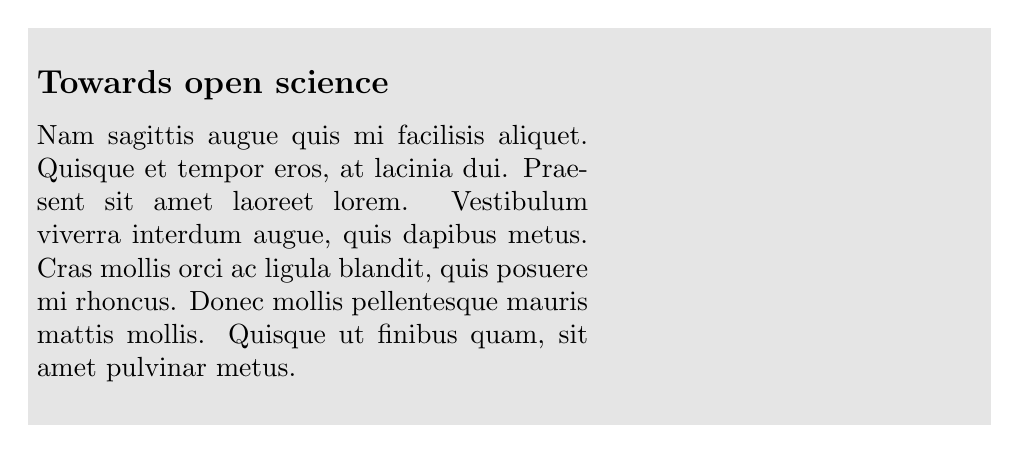
\begin{tikzpicture}[remember picture]
    %\useasboundingbox (0,0) rectangle (3,1);
    \node[xshift=2cm,yshift=7cm, fill=gray!20] at (current page.south west)
       {\begin{minipage}{12cm}
            \begin{minipage}{7cm}
            \bigskip
            \subsection*{Towards open science}

Nam sagittis augue quis mi facilisis aliquet. Quisque et tempor eros, at lacinia dui. Praesent sit amet laoreet lorem. Vestibulum viverra interdum augue, quis dapibus metus. Cras mollis orci ac ligula blandit, quis posuere mi rhoncus. Donec mollis pellentesque mauris mattis mollis. Quisque ut finibus quam, sit amet pulvinar metus.
\bigskip
            \end{minipage}
            
        \end{minipage}
       };
\end{tikzpicture}

\pagebreak


%\FloatBarrier

\section*{Contribution to Publications}
\label{ContPub}


The scientific papers that merge the core of the thesis is as follows:

\bigskip

\textbf{Paper I / Chapter 2}

\medskip

\noindent \hangindent=0.6cm Heistermann, Maik, Irene Crisologo, Catherine C. Abon, Bernard Alan Racoma, Stephan Jacobi, Nathaniel T. Servando, Carlos Primo C. David, and Axel Bronstert. 2013. “Brief Communication ‘Using the New Philippine Radar Network to Reconstruct the Habagat of August 2012 Monsoon Event around Metropolitan Manila.’” Nat. Hazards Earth Syst. Sci. 13 (3): 653–57. https://doi.org/10.5194/nhess-13-653-2013.

\medskip

MH conceptualized the study, together with IC and CCA; NTS and CPCD provided the radar data; MH wrote the software code, and MH and IC carried out the analysis. MH prepared the manuscript, with contributions from all co-authors.

\bigskip

\textbf{Paper II / Chapter 3}

\medskip

\noindent \hangindent=0.6cm Crisologo, Irene, Robert A. Warren, Kai Mühlbauer, and Maik Heistermann. 2018. “Enhancing the Consistency of Spaceborne and Ground-Based Radar Comparisons by Using Beam Blockage Fraction as a Quality Filter.” Atmospheric Measurement Techniques 11 (9): 5223–36. https://doi.org/10.5194/amt-11-5223-2018.

\medskip

IC and MH conceptualized the study. KM, MH, RW, and IC formulated the 3D-matching code based on previous work of RW. IC carried out the analyses; IC and MH the interpretation of results. IC and MH, with contributions from all authors, prepared the manuscript.

\bigskip

\textbf{Paper III / Chapter 4}

\medskip

\noindent \hangindent=0.6cm Crisologo, Irene and Maik Heistermann: Using ground radar overlaps to verify the retrieval of calibration bias estimates from spaceborne platforms, Atmos. Meas. Tech., submitted.

\medskip

IC and MH conceptualized the study and formulated the code for 3D-matching of GRs. IC prepared the scripts for 3-way comparison and carried out the analysis. IC and MH interpreted the results and prepared the manuscript. 




\end{multicols}